\chapter{Technical Approach}
\label{ch:tec}

In this chapter we will explain the technical means by which the objective of this thesis has been approached. Firstly, in section \ref{s:pre} we start talking about the WHAT… (Franka Emika, The \emph{Robot Operating System} (ROS), \emph{Gazebo}). In order to make the robot avoid obstacles with proximity data, obstacles need to be located with respect to the robots’ kinematic chain. In section \ref{s:calibration} we briefly present a framework for automatic kinematic calibration that leverages an IMU to accurately estimate the pose (position and orientation) of skin units along the surface of a robot. In section \ref{s:control} the methods for obstacle avoiding control are presented.

\section{Preliminaries}
\label{s:pre}
\subsection{ROS}

The Robot Operating System (ROS) is an open source robot middleware or robot development environment (RDE), one of many available in the market. Robot middleware \cite{elkady2009middlew} is an abstraction layer that resides between the operating system (OS) and software applications (figure \ref{fig:middleware}). Its purpose is to provide a framework and  take care of several important parts of an application development, so that the developer needs only to build the logic or algorithm as a component.

\begin{figure}[htbp]
    \caption[Robotic middleware]{
        Robotic middleware \cite{elkady2009middlew}
    }
    \begin{center}
    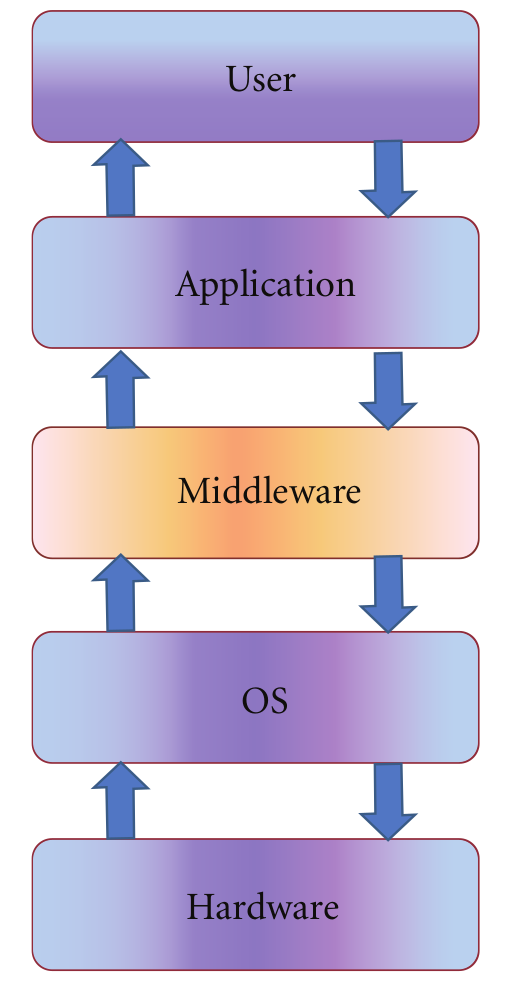
\includegraphics[width=45mm]{figs/middleware.png}
    \end{center}
\label{fig:middleware}
\end{figure}

ROS’s main concept is its runtime graph: a peer-to-peer network of loosely coupled components or nodes that use the ROS communication infrastructure. ROS implements several different means of communication:

\begin{itemize}
    \item
\end{itemize}

Example

\begin{figure}[htbp]
    \caption[ROS graph]{
        ROS graph
    }
    \begin{center}
    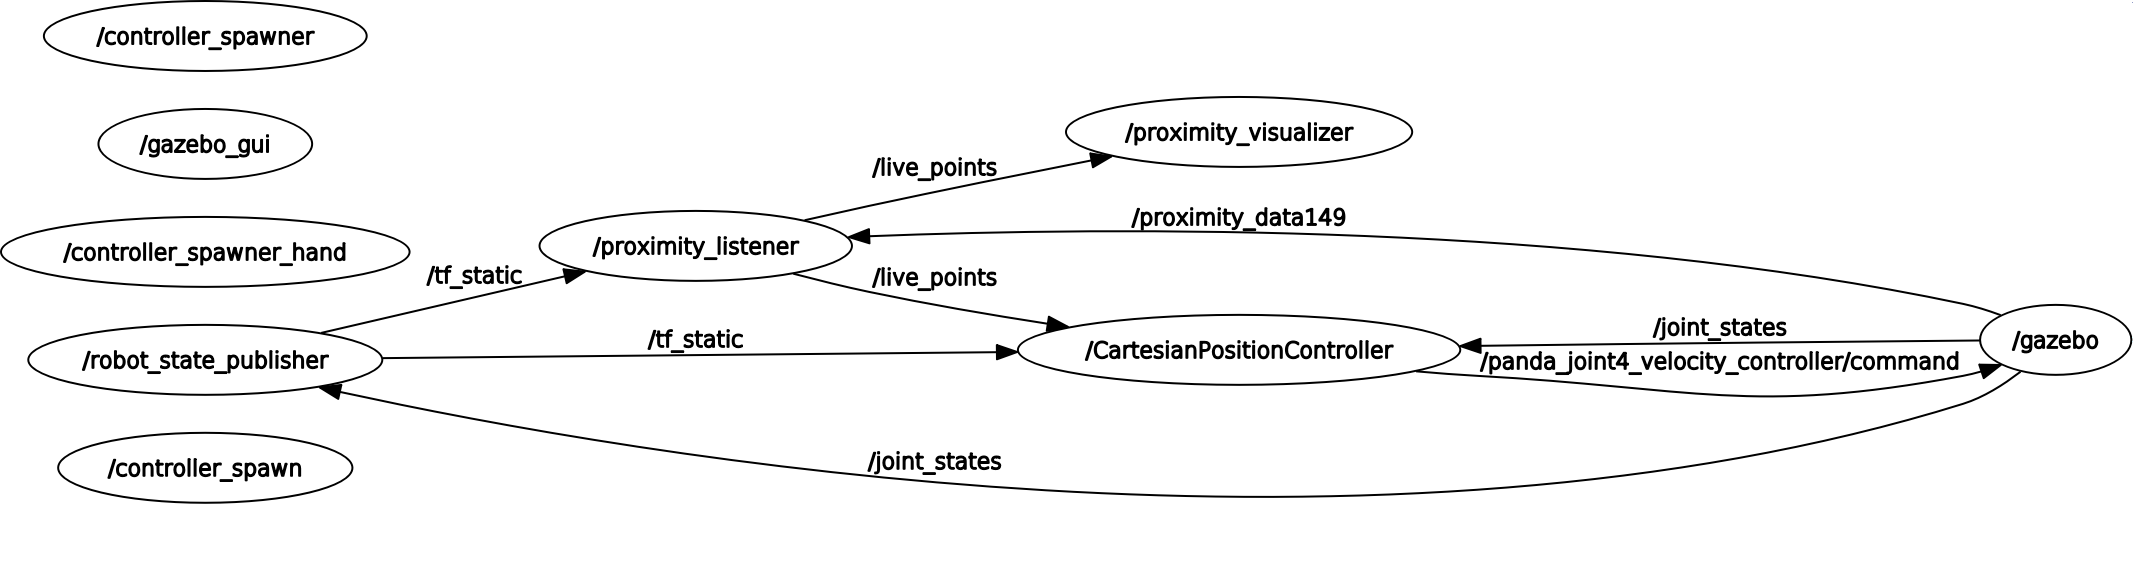
\includegraphics[width=165mm]{figs/rosgraph.png}
    \end{center}
\label{fig:rosgraph}
\end{figure}

The ROS Master enables nodes to find each other and to communicate. It also holds the parameter server, which provides a central storage location for data that is relevant for several nodes. It serves, broadly speaking, as a place where global variables can be stored and retrieved by nodes. Examples of things that are stored in the parameter server are PID control parameters, the robot’s urdf description and frequencies at which different components that live in the graph work.

Last, it should be mentioned that despite the fact that ROS is widely used in the academic context, it is lacking reliability and robustness safety critical systems in industrial or commercial contexts require. Some of the industrial fields, such as the automotive and the aerospace, have their own standards for development of safety-critical software. These standards need to be certified for every software component written in any of these fields. ROS was not developed to any of these standards and it actually depends on many libraries that were not developed to this standards. ROS 2, in contrast, is based on components that are safety-certified (DDL) and makes ROS 2 certifiable. Indeed, Apex.AI is working on Apex.OS: an API compatible to ROS 2 that is being certified ISO 26262 for safe automotive applications \cite{apexOS}.

\subsection{Panda robot by Franka Emika}

\section{Kinematic Calibration}
\label{s:calibration}

We present a framework for automatic kinematic calibration that leverages an
IMU to accurately estimate the pose (position and orientation) of skin units,
of arbitrary number, along the surface of a robot.

To automatically locate skin units along the surface of a robot,
we utilize the angular velocity and linear acceleration measurements from the IMUs.
Our optimization algorithm estimates the pose (position and orientation) of an SU
using \textit{modified Denavit-Hartenberg (DH) parameters} [1] as illustrated in figure \ref{fig:calibration_theory}.
The pose of each SU is estimated by six DH parameters with respect to the previous
joint in the kinematic chain: four parameters from the joint to a virtual joint,
and two additional parameters from the virtual joint to the SU (other two parameters are set to $0$).
A virtual joint is located within the link that is orthogonal to the joint’s $z$ axis and the SU’s $z$ axis.
This solution is necessary to adhere to the Denavit-Hartenberg notation,
so that each transformation can be expressed with no more than four parameters.

\begin{figure}[htbp]
    \caption[Calibration theory]{
        Depiction of multiple skin units (S) placed on the robots links (L) and separated by joints (J).
        We estimate the Denavit-Hartenberg parameters of each joint in order to calculate the pose of each skin unit along the surface of the robot.
    }
    \begin{center}
    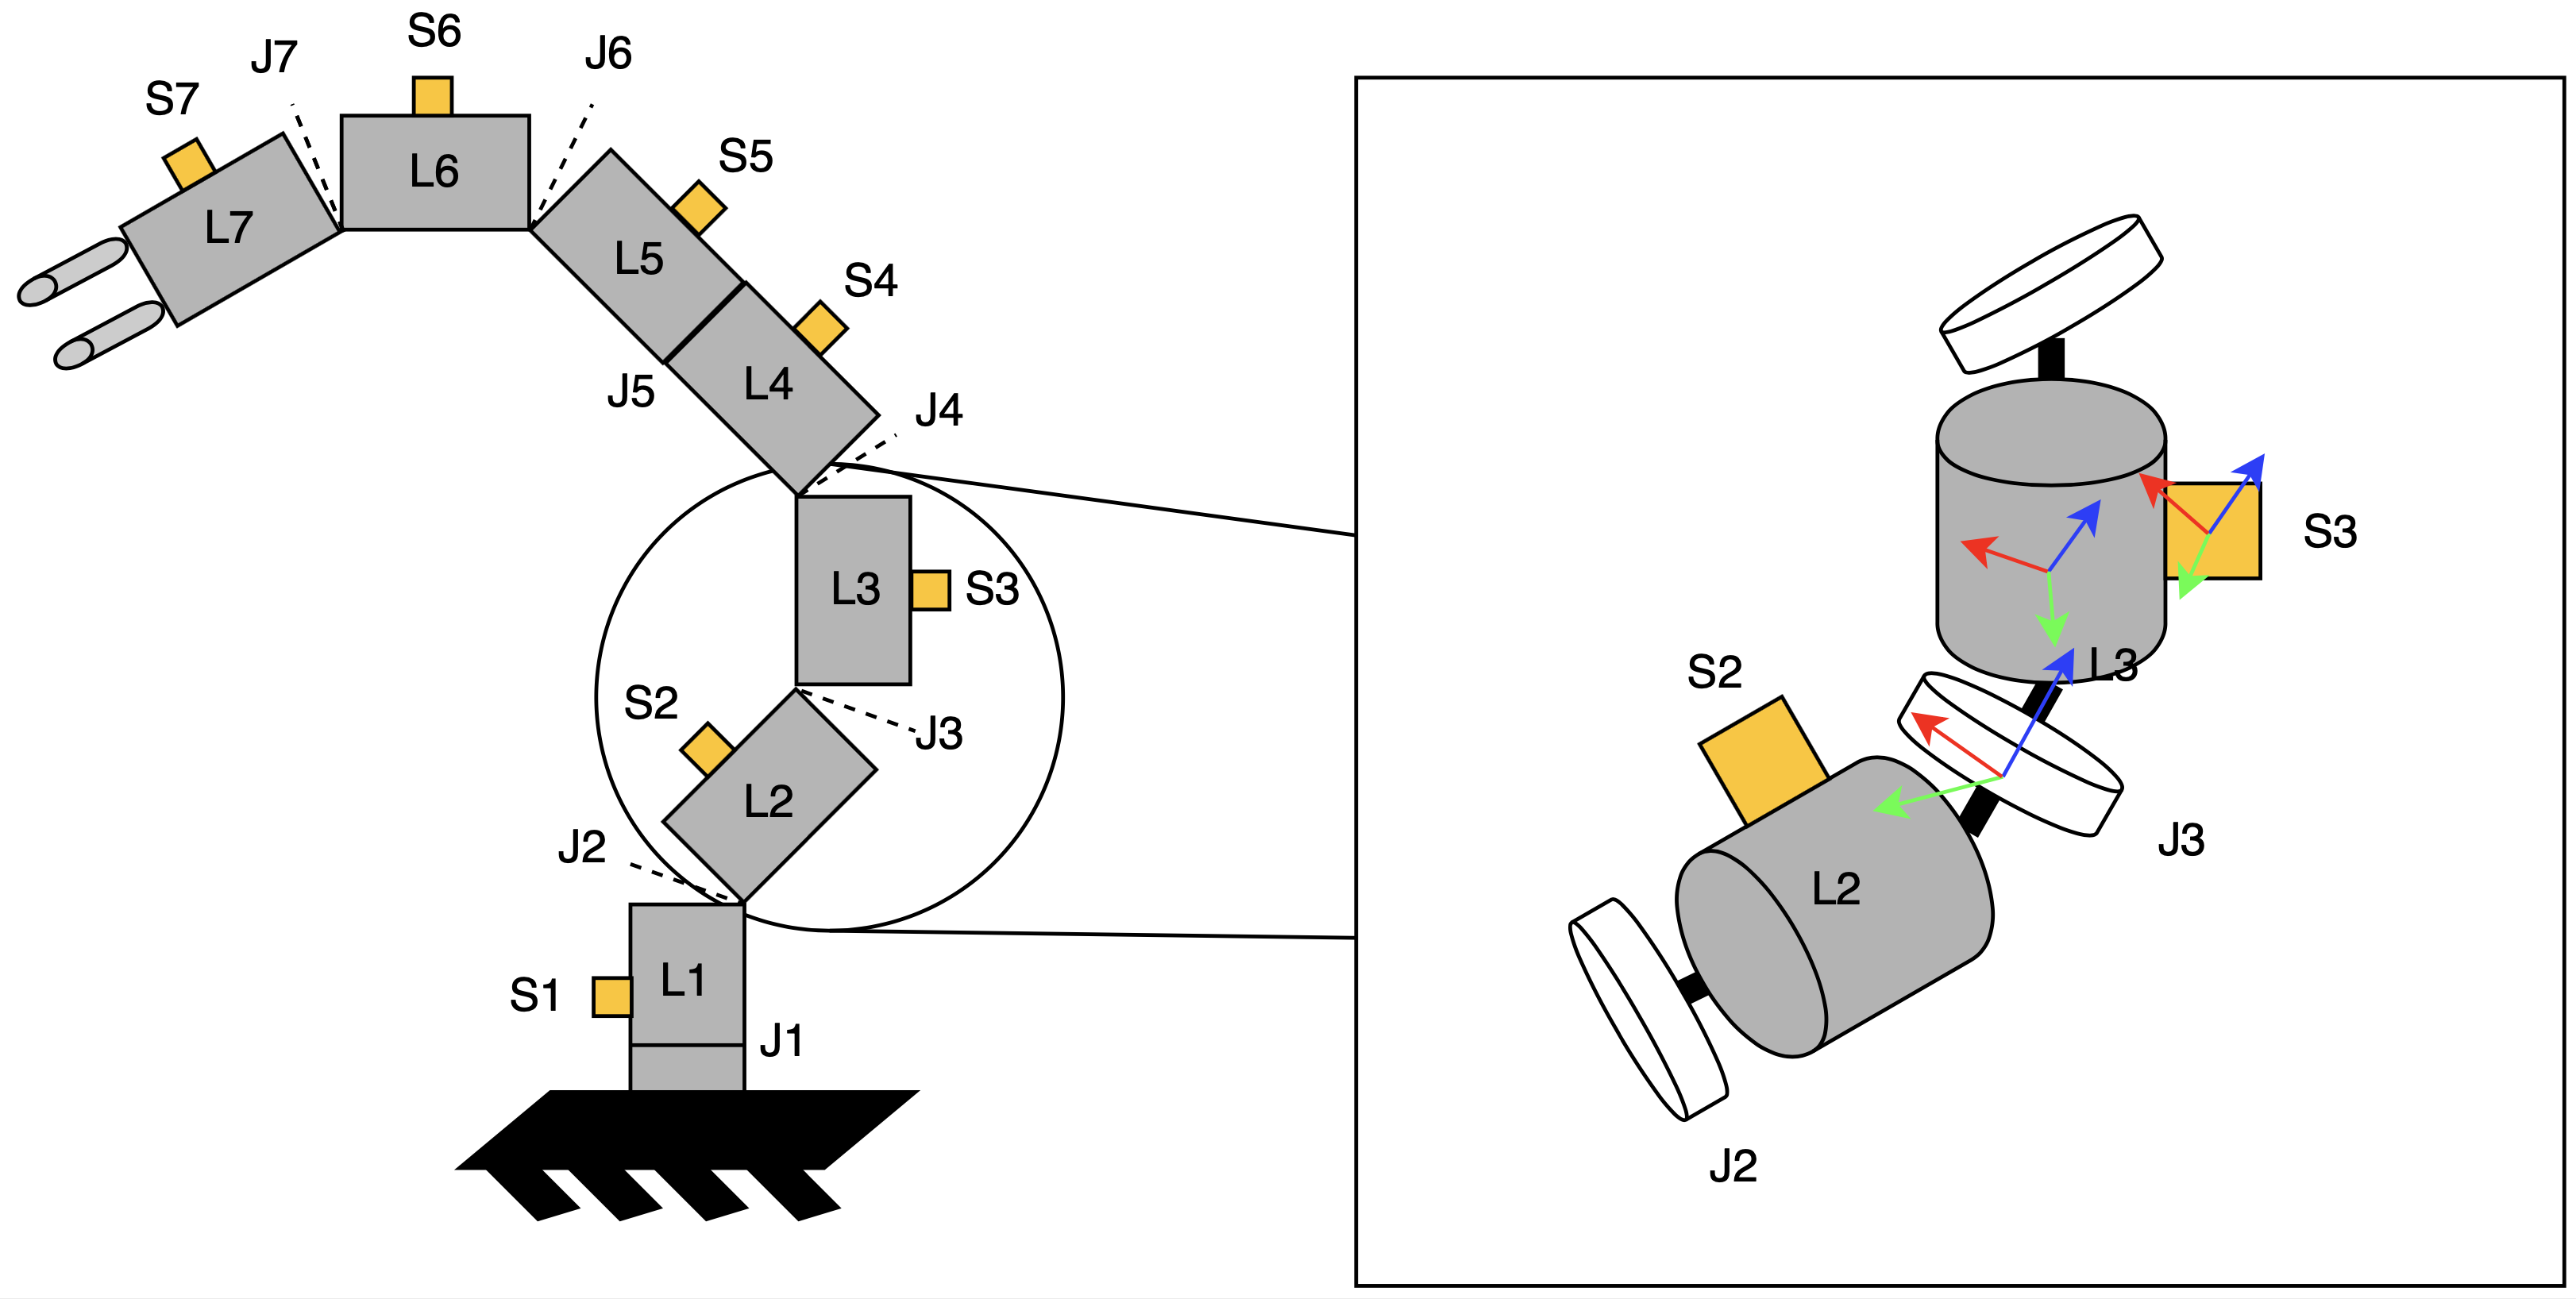
\includegraphics[width=140mm]{figs/calibration_theory.png}
    \end{center}
\label{fig:calibration_theory}
\end{figure}

Our optimization algorithm is composed of the following \textbf{four steps}:

\begin{enumerate}
    \item \paragraph{Initialize a kinematic chain with randomized values.}
    We represent each skin unit coordinate using a transformation matrix.
    $${}^0T_{SU_i} = {}^0T_1 \cdot {}^1T_2 \dots {}^{i-1}T_i \cdot {}^i T_{SU_i}, \quad \forall i$$
    , where:
    $$
    {}^{i}T_{i+1} =
        \left[ \begin{array}{c|c}
            {}^{i}R_{i+1} & {}^{i}\mathbf{p}_{i+1} \\
            \hline
            \mathbf{0} & 1 \\
        \end{array}\right].
    $$

    \item \paragraph{Collect Data.}
    First, static forces applied to the IMU (that is, the constant acceleration due to gravity)
    are measured and compensated for.
    Then, each reference joint is moved through its operational range in a constant rotation pattern
    and the resulting acceleration as measured by the IMU is stored.

    \item \paragraph{Define an error function.}
    Acceleration exerted on each SU ${}^{SU_i}a_{u,d}$ can be estimated as a composition of local acceleration,
    tangential acceleration and centripetal acceleration:
    $$^{RS}\mathbf{a}_{t a n_{u, d}} = ^{R S} \mathbf{\alpha}_{d} \times^{R S} \mathbf{r}_{u, d}$$

    $$^{RS}\mathbf{a}_{cp_{u, d}} = ^{R S} \mathbf{\omega}_{d} \times\left(^{R S} \mathbf{\omega}_{d} \times^{R S} \mathbf{r}_{u, d}\right)$$

    $$^{SU_{i}}\mathbf{a}_{u, d} = ^{SU_{i}}\underline{R}_{R S} \cdot\left(^{R S} \mathbf{g}+^{R S} \mathbf{a}_{t a n_{u}, d}+^{R S} \mathbf{a}_{c p_{u, d}}\right).$$
    Angular velocity $\mathbf{\omega}$ and angular acceleration $\mathbf{\alpha}$ are measured during data collection, whereas rotation matrix $R$ and position vector $\mathbf{p}$ can be computed using the current estimated DH parameters.

    One example error function could be seen as the error between the measured accelerations from the IMUs and the estimated accelerations using the kinematic chain model for $n_{pose}$ poses [2]:
    $$E = \sum_{i=1}^{n_{pose}} \sum_{j=1}^{n_{joint}} ||a^{model}_{i,j} - a^{IMU}_{i,j}||^2$$

    \item \paragraph{Minimize the error function with a global optimizer.}
    A global optimizer optimizes the DH parameters by minimizing the chosen error function. We combine several different error functions to estimate both rotational and translational parameters. The final result in simulation can be seen in figure \ref{fig:calibration_result}.

\end{enumerate}

\begin{figure}[htbp]
    \caption[Calibration result]{
    Calibrated IMU positions on a simulated Franka Emika Panda robot.
    }
    \begin{center}
    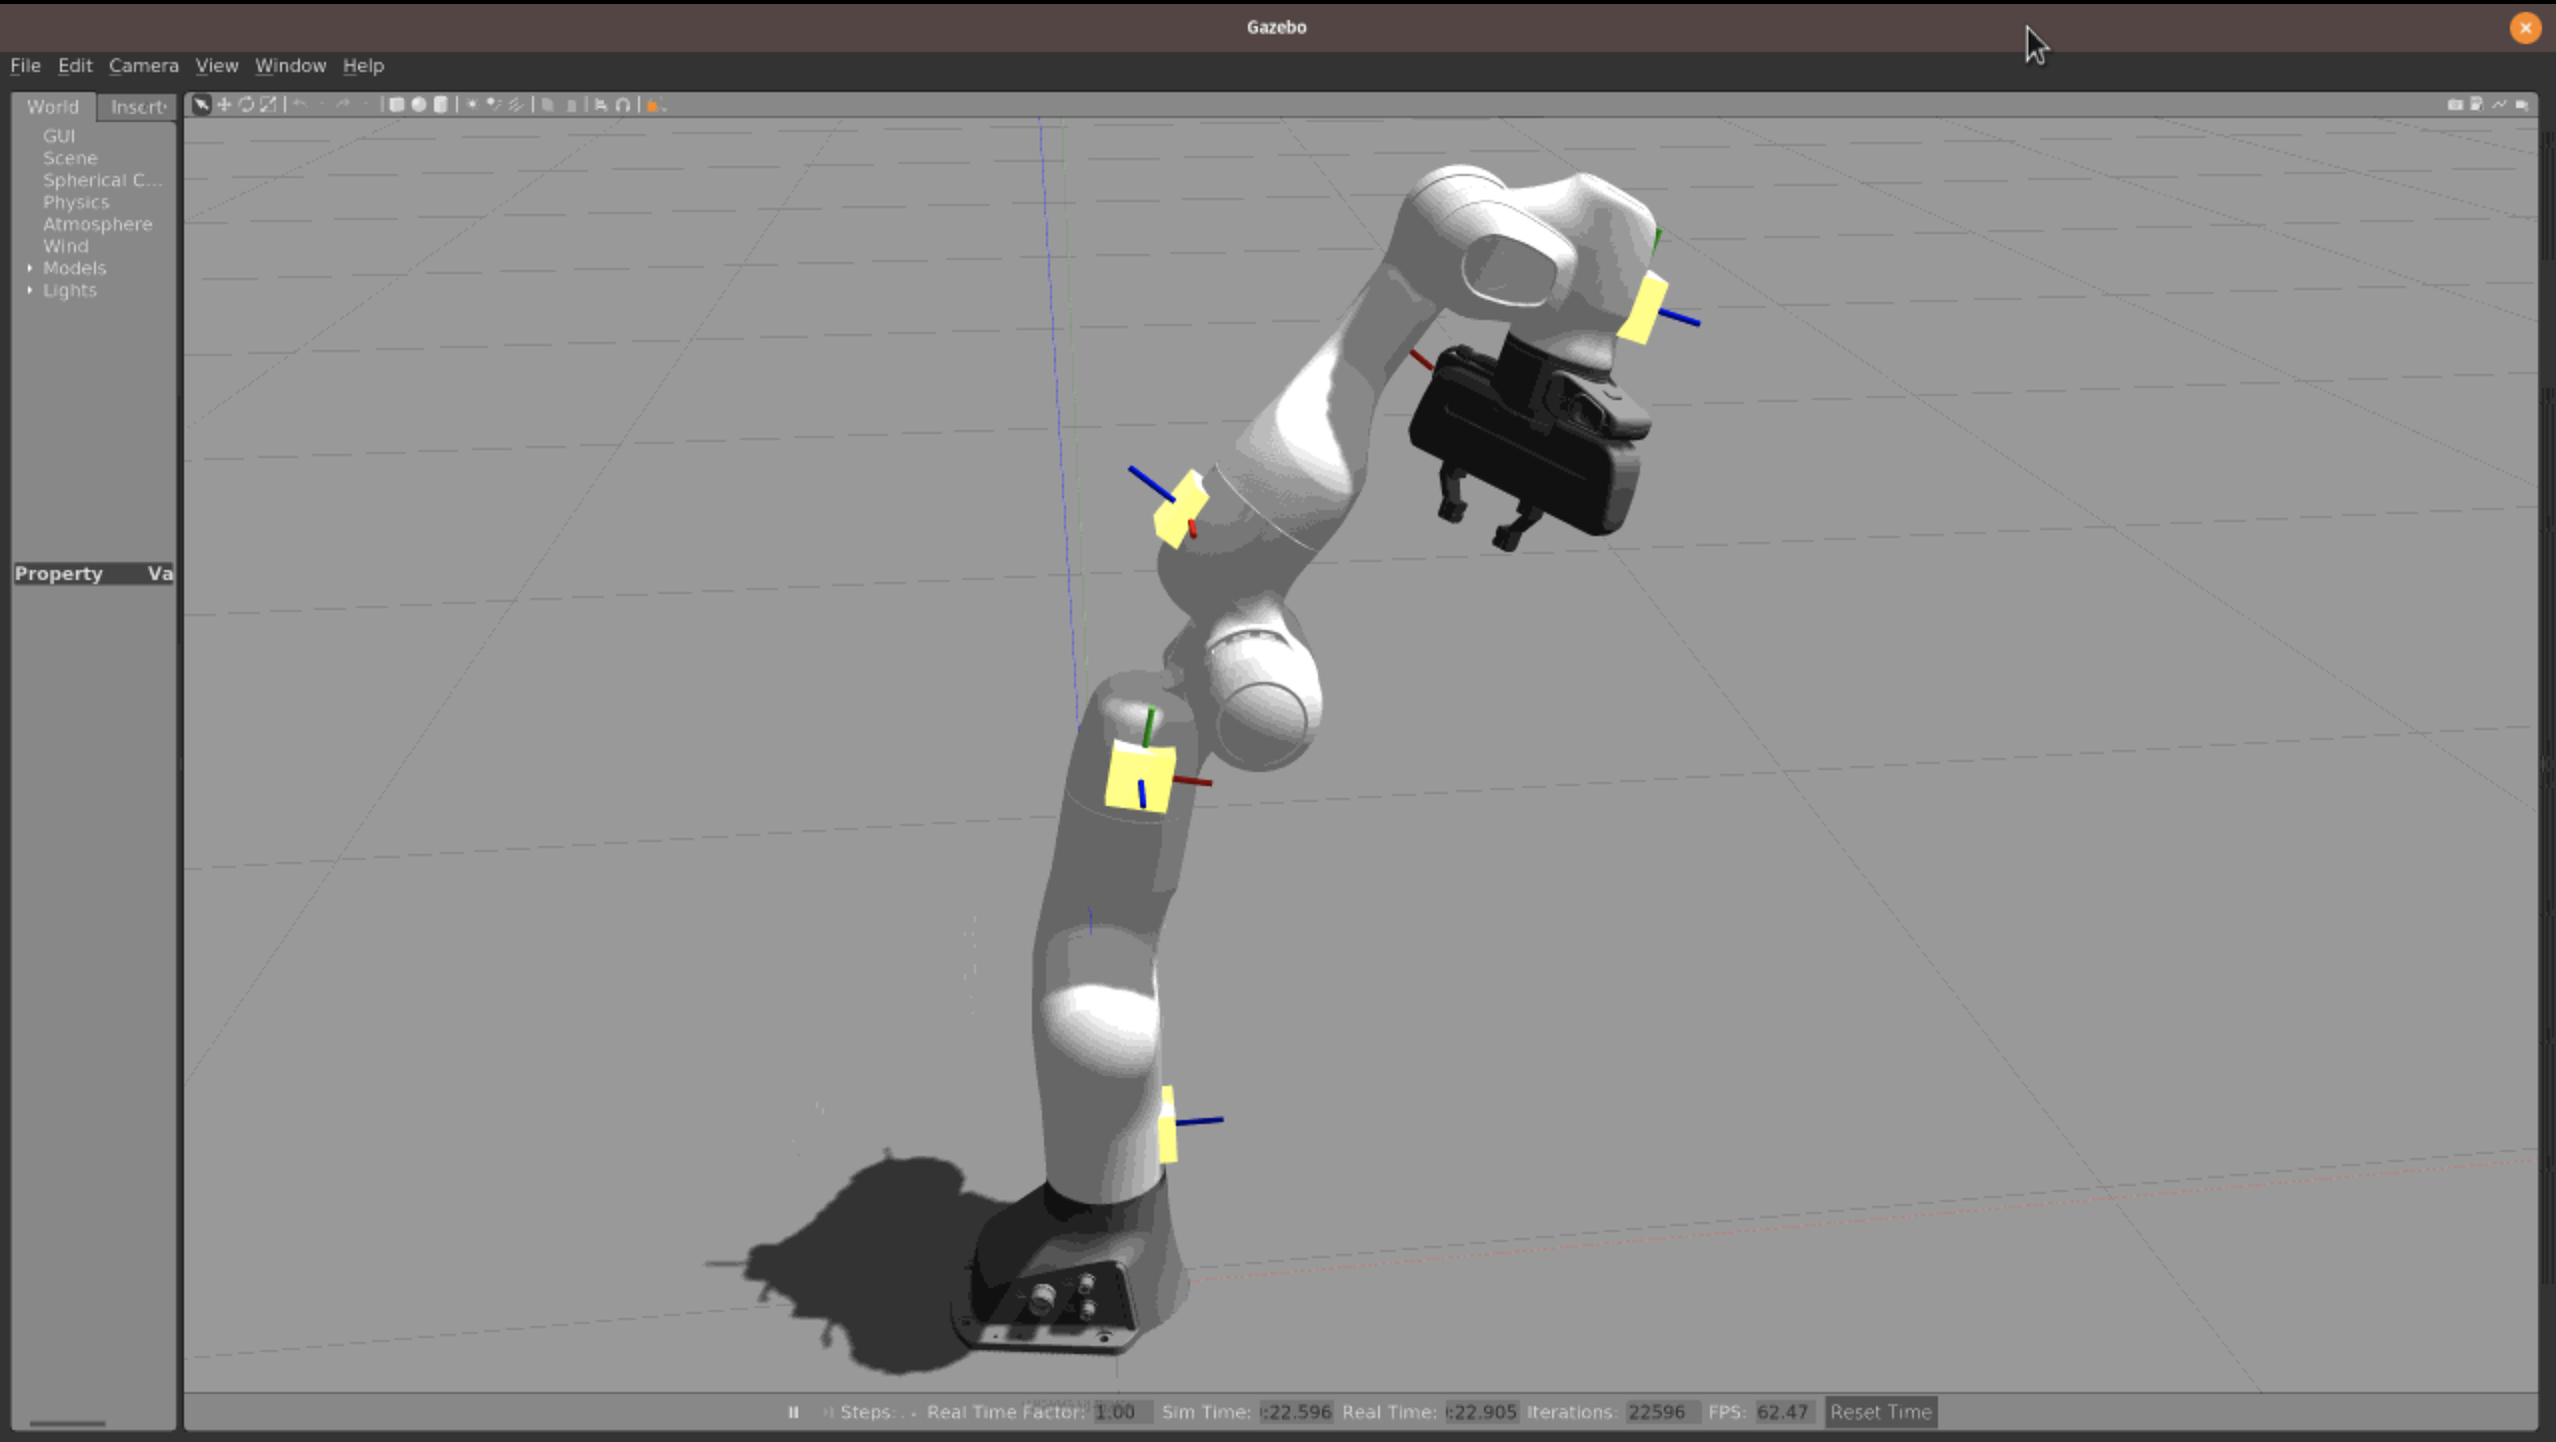
\includegraphics[width=140mm]{figs/calibration_result.png}
    \end{center}
\label{fig:calibration_result}
\end{figure}

\section{Control}
\label{s:control}

Jacobian

Inverse kinematics

Linear system with redundancy
